\chapter{希格斯标度、跑动耦合与等级问题}

\lectureoverview{最后一讲从标准模型之外出发，展望统一、超对称与规范等级问题。为了看清希格斯场为何处于这些问题的中心，我们首先重建狄拉克拉格朗日量，并表明费米子质量混合了左、右手征。手征弱相互作用禁止该质量作为裸项存在；只有希格斯场获得真空值之后，规范不变的汤川耦合才提供质量。随后我们从希格斯势推导出该真空值，追问为何所有已知基本粒子质量都系于这一个小标度，并以超导性作为物理类比。课间休息之后，本讲从导体与电介质屏蔽发展出重整化，把论证带入量子电动力学与量子色动力学，追踪规范耦合走向统一，并从短距离引力推导普朗克标度。电弱标度于是重新作为唯一无法解释的小数出现。}

\section{标准模型之外等待的问题}

这里并不把标准模型呈现为一个封闭的目录。今晚开始时，我想说明下一门课程将走向何处。该理论有的是困难而非逻辑悖论：规范等级问题、超对称可能扮演的角色，以及统一问题。三个规范因子
\begin{equation}
  SU(3)_c\times SU(2)_L\times U(1)_Y
  \label{eq:l10-standard-model-group}
\end{equation}
分别描述强、弱和超荷相互作用。它们会不会是一个更大群的子群？一个常被研究的可能性是
\(SU(5)\)，其中夸克与轻子占据共同的表示。自然界是否采用这一特定构造则是另一个问题。重要的线索是，那些看似分离的结构极为整齐地嵌入一个更大的数学结构之中。

大型强子对撞机的建造部分是为了揭示解决这些问题的物理。在2010年，它最直接的目标是希格斯玻色子。发现希格斯粒子绝不意味着只是往表格里添加一个粒子。希格斯粒子是通过一组相互关联的性质来确认的：其真空值赋予弱矢量玻色子和费米子质量，而其涨落则以确定的强度耦合到这些相同的粒子。耦合方式错误的共振态不会是标准模型希格斯粒子。\editorialnote{本讲早于2012年的发现。所观测到的约\(125\,\mathrm{GeV}\)标量粒子，在目前精度内具有标准模型希格斯粒子所预期的自旋、宇称和耦合模式。截至2026年，尚未观测到低能超对称粒子。这些后来事实更新了历史背景，却不改变当时在教室里展开的论证。}

进入该论证的路径并非始于希格斯势，而是始于狄拉克方程。我们需要确切理解费米子质量做了什么，然后才能追问它从何而来。

\section{从狄拉克方程到其拉格朗日量}

\subsection{较早的狄拉克记号}

在最初引入狄拉克方程时所使用的哈密顿量记号中，其结构为
\begin{equation}
  i\partial_t\psi
  =
  \left(-i\alpha^i\partial_i+\beta m\right)\psi .
  \label{eq:l10-dirac-hamiltonian}
\end{equation}
符号和\(i\)的因子取决于约定，而现场板书暂时省略了其中一些。不变的内容是含导数项与不含导数的质量项之间的分离。

\begin{figure}[htbp]
\centering
\includegraphics[width=0.82\textwidth]{lecture_10_figure_02.png}
\caption{较早的\(\alpha,\beta\)记号下的狄拉克方程与拉格朗日量。板书是从结构上使用，而非作为固定的符号约定。}
\lectureframe{00:05:52}
\label{fig:l10-dirac-alpha-beta}
\end{figure}

为了得到一个其变分给出狄拉克方程的作用量，将方程乘以\(\psi^\dagger\)。把每一项移到一侧便不再需要等号，这引出了当晚的一个小小数学玩笑：一旦方程被写成某个恒为零的表达式，等号就完成了它的使命。相应的一阶拉格朗日量可示意性地写为
\begin{equation}
  \mathcal L
  =
  \psi^\dagger
  \left(i\partial_t+i\alpha^i\partial_i-\beta m\right)\psi ,
  \label{eq:l10-dirac-old-lagrangian}
\end{equation}
这里默认一致的度规约定固定了相对符号。

导数项把一个激发从一个时空点移动到邻近的时空点，并在此过程中旋转其旋量分量。在点阵图像中，它们是跃迁项。相比之下，质量项在同一点吸收并重新发射费米子。它不含导数。这一局域操作很快将显现为两种手性之间的反复转换。

\begin{classroomqa}
\audiencequestion{是否应在
\(\psi^\dagger\)之后放置\(\gamma^0\)？\lecturetimestamp{00:05:59}}
\lecturerresponse{在刚才写出的非协变形式中并不需要。但这个问题直接指向了协变记号。用\(\bar\psi=\psi^\dagger\gamma^0\)定义狄拉克伴随；于是\(\gamma^0\)确实被内置于位于左侧的那个对象之中。}
\end{classroomqa}

\subsection{协变形式}

设
\begin{equation}
  \bar\psi\equiv\psi^\dagger\beta
  =\psi^\dagger\gamma^0,
  \qquad
  \gamma^0\equiv\beta,
  \qquad
  \gamma^i\equiv\beta\alpha^i .
  \label{eq:l10-dirac-adjoint}
\end{equation}
由于\(\beta^2=1\)，乘以\(\beta\)可在两种记号之间自由转换。时间导数变为
\(\bar\psi\gamma^0\partial_0\psi\)，空间导数变为
\(\bar\psi\gamma^i\partial_i\psi\)，结果为
\begin{equation}
  \boxed{\mathcal L_D
  =\bar\psi\left(i\gamma^\mu\partial_\mu-m\right)\psi .}
  \label{eq:l10-covariant-dirac}
\end{equation}

\begin{figure}[htbp]
\centering
\includegraphics[width=0.82\textwidth]{lecture_10_figure_03.png}
\caption{协变改写：\(\bar\psi=\psi^\dagger\gamma^0\)、
\(\gamma^i=\beta\alpha^i\)，以及紧凑的狄拉克拉格朗日量。}
\lectureframe{00:10:17}
\label{fig:l10-dirac-covariant}
\end{figure}

这一记号揭示了每个双线性量的洛伦兹性质。
\(\bar\psi\psi\)是标量，而
\(\bar\psi\gamma^\mu\psi\)是四维矢量。紧凑表达式不仅仅比\(\alpha,\beta\)形式更漂亮；它还告诉我们各个部分如何变换。

\begin{classroomqa}
\audiencequestion{紧凑表达式最左侧的旋量是否本应为\(\bar\psi\)？\lecturetimestamp{00:09:39}}
\lecturerresponse{是的。缺失的横杠已在黑板上补回。这很重要：
\(\bar\psi\)不是\(\psi^\dagger\)，而是
\(\psi^\dagger\gamma^0\)。}
\end{classroomqa}

\section{手征性与狄拉克质量实际起的作用}

除\(\gamma^0,\gamma^1,\gamma^2,\gamma^3\)之外，定义
\begin{equation}
  \gamma^5
  =i\gamma^0\gamma^1\gamma^2\gamma^3,
  \qquad
  (\gamma^5)^2=1 .
  \label{eq:l10-gamma-five}
\end{equation}
此处出现的因子\(i\)是主要度规为负号的闵可夫斯基度规的标准约定。本征值为\(+1\)和\(-1\)，相应的投影算符为
\begin{equation}
\begin{aligned}
  P_L&=\frac{1-\gamma^5}{2},
  &
  P_R&=\frac{1+\gamma^5}{2},
  \\
  \psi_L&=P_L\psi,
  &
  \psi_R&=P_R\psi .
\end{aligned}
  \label{eq:l10-chiral-projectors}
\end{equation}

\begin{classroomqa}
\audiencequestion{既然没有\(\gamma^4\)，为什么这个额外的矩阵被称为\(\gamma^5\)？它的本征值描述的是螺旋度吗？\lecturetimestamp{00:10:42}}
\lecturerresponse{这个名字是历史性的：它是由四个时空伽马矩阵之积构成的额外矩阵。它的本征值标记的是手征性，一般不是螺旋度。对于无质量粒子，这两个概念可以适当地等同起来，这正是相关说法容易被混淆的原因，但手征性才是弱规范理论所需的洛伦兹表示标签。}
\end{classroomqa}

动能项保持手征性。看出这一点的一个有用方式是\(\{\gamma^\mu,\gamma^5\}=0\)，因此它分解为
\begin{equation}
  \bar\psi i\gamma^\mu\partial_\mu\psi
  =
  \bar\psi_L i\gamma^\mu\partial_\mu\psi_L
  +
  \bar\psi_R i\gamma^\mu\partial_\mu\psi_R .
  \label{eq:l10-chiral-kinetic}
\end{equation}
标量双线性量的行为则不同：
\begin{equation}
  \bar\psi\psi
  =
  \bar\psi_L\psi_R+\bar\psi_R\psi_L .
  \label{eq:l10-chiral-mass}
\end{equation}

\begin{figure}[htbp]
\centering
\includegraphics[width=0.80\textwidth]{lecture_10_figure_04.png}
\caption{黑板上将标量双线性量分解为从左到右和从右到左的部分。}
\lectureframe{00:15:38}
\label{fig:l10-chiral-decomposition}
\end{figure}

因此，狄拉克质量是一种局域的手征翻转操作：
\begin{equation}
  \psi_L\longleftrightarrow\psi_R .
\end{equation}
无质量费米子可以以确定的手征性传播。有质量费米子则不能停留在单一手征扇区中，因为质量项不断混合两者。这种转换竟与惯性有关，或许令人惊讶，但这恰恰是费米子静止质量的相对论场论形式。

\section{为什么弱对称性禁止裸费米子质量}

带电弱流是纯左手手征的。讲座首先提到\(Z\)，随后将说法更正为\(W^\pm\)：\(Z\)耦合是手征的且不相等，但并非对每个右手手征费米子都简单地不存在。准确的表述是
\begin{equation}
  \mathcal L_{\mathrm{cc}}
  =
  -\frac{g}{\sqrt2}
  \left(\bar u_L\gamma^\mu d_L
  +\bar\nu_L\gamma^\mu e_L\right)W^+_\mu
  +\mathrm{h.c.}
  \label{eq:l10-charged-current}
\end{equation}
左手费米子按\(SU(2)_L\)二重态变换；右手带电费米子按单态变换。

现在将这些变换规则与
\eqref{eq:l10-chiral-mass}比较。诸如
\(\bar e_L e_R\)这样的项吸收一个携带某组电弱量子数的对象，并发射出另一个携带不同量子数的对象。它本身不是规范不变的。因此，熟悉的狄拉克质量作为电弱拉格朗日量中的裸项是非法的。

这才是正确的解释顺序。费米子质量并非先被插入，然后再与希格斯粒子作装饰性关联。规范对称性首先去掉了显然的质量项。然后希格斯场被迫携带缺失的量子数。

\subsection{希格斯作为电荷载体}

设希格斯场按超荷为
\(+\tfrac12\)的\(SU(2)_L\)二重态变换：
\begin{equation}
  H=
  \begin{pmatrix}
    H^+\\ H^0
  \end{pmatrix},
  \qquad
  \widetilde H=i\sigma^2H^* .
  \label{eq:l10-higgs-doublet}
\end{equation}
讲座将群指标保持为示意性的，并称该场为\(\phi\)。在该记号下，汤川项具有形式
\begin{equation}
  \mathcal L_Y
  =
  -G_Y\left(
    \bar\psi_L\phi\psi_R+
    \bar\psi_R\phi^\dagger\psi_L
  \right).
  \label{eq:l10-yukawa-schematic}
\end{equation}
希格斯场带走了裸手征翻转所无法守恒的弱荷。

完整的一代标准模型表达式明确地体现了同样的记账：
\begin{equation}
  \mathcal L_Y
  =
  -y_d\bar Q_LHd_R
  -y_u\bar Q_L\widetilde H u_R
  -y_e\bar L_LHe_R
  +\mathrm{h.c.}
  \label{eq:l10-yukawa-full}
\end{equation}
每一项都是规范不变的，且每种费米子都带有各自的无量纲汤川耦合。

\begin{figure}[htbp]
\centering
\includegraphics[width=0.80\textwidth]{lecture_10_figure_05.png}
\caption{希格斯辅助的手征翻转和对称破缺势一起出现在黑板上。}
\lectureframe{00:18:54}
\label{fig:l10-yukawa-potential-board}
\end{figure}

\section{一个相互作用同时成为质量和希格斯耦合}

自然界选择的是一个中性希格斯分量不为零的真空。在讲义所用的示意性实场记号中，
\begin{equation}
  \phi=F+\mathcal H ,
  \label{eq:l10-f-plus-h}
\end{equation}
其中 \(F\) 是不涨落的真空平移，而 \(\mathcal H\) 是传播的希格斯涨落。将其代入
\eqref{eq:l10-yukawa-schematic} 得到
\begin{align}
  \mathcal L_Y
  ={}&
  -G_YF
  \left(\bar\psi_L\psi_R+\bar\psi_R\psi_L\right)
  \notag\\
  &-G_Y\mathcal H
  \left(\bar\psi_L\psi_R+\bar\psi_R\psi_L\right).
  \label{eq:l10-yukawa-split}
\end{align}
第一行是狄拉克质量，第二行是与物理希格斯量子的相互作用：
\begin{equation}
  m_f=G_YF
  \qquad\hbox{in the lecture's normalization.}
  \label{eq:l10-mass-lecture-normalization}
\end{equation}

在标准的标准模型归一化下，
\begin{equation}
\begin{aligned}
  H(x)&=\frac{1}{\sqrt2}
  \begin{pmatrix}
    0\\ v+h(x)
  \end{pmatrix},
  \\
  m_f&=\frac{y_fv}{\sqrt2},
  \\
  \mathcal L_{hff}&=-\frac{m_f}{v}h\bar f f,
\end{aligned}
  \label{eq:l10-standard-higgs-normalization}
\end{equation}
其中 \(v\simeq246\,\mathrm{GeV}\)。讲义中粗略的
\(F\sim200\,\mathrm{GeV}\) 就是同一个电弱能标，只是省略了归一化细节。

测得的 \(W\) 和 \(Z\) 质量确定了能标 \(F\)。测得的费米子质量随后确定了汤川耦合。电子的耦合极小；顶夸克的耦合为 1 的量级。如果这就是该机制的全部作用，那么我们不过是每个费米子引入一个未知数，再把同样的信息读出来而已。

但 \eqref{eq:l10-yukawa-split} 的第二行是新的实验内容。它表明费米子可以发射或吸收一个希格斯粒子，而在交叉道中解读，则表明希格斯粒子可以衰变为费米子—反费米子对。示意性地，
\begin{equation}
\begin{aligned}
  \mathcal M(h\to f\bar f)&\propto y_f,
  \\
  \Gamma(h\to f\bar f)
  &=
  N_c\frac{y_f^2m_h}{16\pi}
  \\
  &\quad\times
  \left(1-\frac{4m_f^2}{m_h^2}\right)^{3/2},
\end{aligned}
  \label{eq:l10-higgs-fermion-width}
\end{equation}
在树图阶。这里对夸克 \(N_c=3\)，对轻子 \(1\)。费米子质量越大，汤川耦合就越大，前提是该衰变在运动学上允许。这并不意味着每个重道都占主导：色因子、相空间、圈图诱导的道以及衰变到矢量玻色子也都有影响。它意味着费米子耦合本身与质量成正比。

\begin{classroomqa}
\audiencequestion{如果不做所有技术细节，人们实际上会如何预言希格斯衰变时间？\lecturetimestamp{00:25:32}}
\lecturerresponse{相互作用给出一个哈密顿矩阵元。画出相应的费曼图，计算其跃迁振幅，将振幅平方，并对所有允许的末态求和或积分。结果就是衰变率。寿命是总宽度的倒数，\(\tau=\hbar/\Gamma_{\mathrm{tot}}\)。这与自量子场论早期发展以来粒子计算中所用的量子力学逻辑相同。}
\end{classroomqa}

在讲课时，这种希格斯唯象学仍然只是预言，而非直接观测。\(W\) 和 \(Z\) 的自相互作用已经对规范结构提供了严格的检验；希格斯粒子及其直接耦合仍有待发现。历史上的不确定性应当记录在案。后来的结果也应当如此：发现了一个类似希格斯的粒子，而对其耦合的测量如今检验的正是这里所发展的同一套产生质量的机制。

\section{选择 F 的势}

真空平移并不是在写出汤川耦合之后手工选定的。它由希格斯势决定。对于穿过完整二重态的一个实截面，取
\begin{equation}
  V(\phi)
  =
  -\frac{\mu^2}{2}\phi^2
  +\frac{\lambda}{4}\phi^4,
  \qquad
  \mu^2>0,\quad\lambda>0.
  \label{eq:l10-real-higgs-potential}
\end{equation}
在 \(\phi=0\) 附近，负的二次项形成一个倒置的抛物线。把 \(\mu\) 称为虚质量，只是说原点不稳定的一种简写；它并不意味着围绕真实真空的物理希格斯激发具有虚质量。

仅二次项会使场无界地增大，从而不留下最低能量态。正的四次项最终会占主导，使势向上弯。奇数次幂会破坏玩具模型中的
\(\phi\mapsto-\phi\) 对称性。四次项是第一个偶的稳定化相互作用，而且在四维时空中，是具有无量纲耦合的最高次多项式标量相互作用。

求导：
\begin{align}
  \frac{dV}{d\phi}
  &=-\mu^2\phi+\lambda\phi^3
  \notag\\
  &=\phi\left(-\mu^2+\lambda\phi^2\right).
  \label{eq:l10-potential-derivative}
\end{align}
驻点 \(\phi=0\) 是不稳定的顶点。两个极小值满足
\begin{equation}
  \boxed{F^2=\frac{\mu^2}{\lambda}},
  \qquad
  F=\frac{\mu}{\sqrt\lambda}
  \label{eq:l10-vacuum-value}
\end{equation}
对于这种实场约定。

\begin{figure}[htbp]
\centering
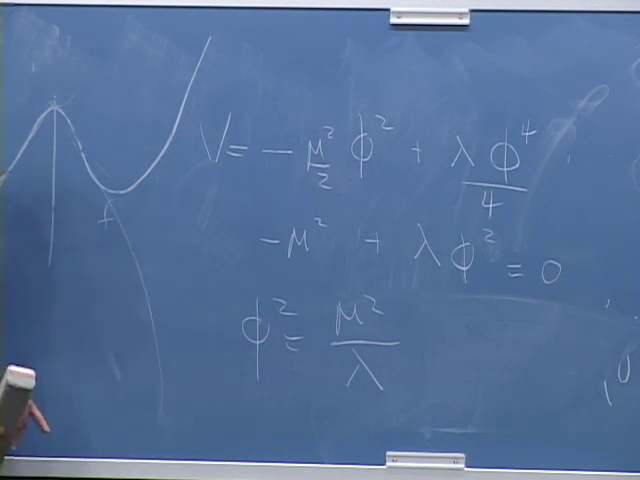
\includegraphics[width=0.84\textwidth]{lecture_10_figure_06.png}
\caption{黑板上完成的极小化：
\(V=-\mu^2\phi^2/2+\lambda\phi^4/4\)、
\(V'=0\) 和 \(\phi^2=\mu^2/\lambda\)。}
\lectureframe{00:34:32}
\label{fig:l10-higgs-minimization}
\end{figure}

插入因子 \(1/2\) 和 \(1/4\) 正是为了使它们在求导时消失。在原点附近，\(\phi^4\) 小于
\(\phi^2\)；在大场值处它增长得更快并使系统稳定。这种简单的竞争产生了双势阱。

量纲也澄清了文字记录中一处短暂的口误。
\(\lambda\) 在四维时空中是无量纲的，而 \(\mu\)
和 \(F\) 具有质量的量纲。展开 \(\phi=F+\mathcal H\)，势的曲率给出
\begin{equation}
  m_{\mathcal H}^2
  =
  \left.\frac{d^2V}{d\phi^2}\right|_{\phi=F}
  =
  -\mu^2+3\lambda F^2
  =
  2\mu^2
  =
  2\lambda F^2.
  \label{eq:l10-higgs-curvature}
\end{equation}
在完整的标准模型记号中，
\(V(H)=-\mu^2H^\dagger H+\lambda(H^\dagger H)^2\)，同样有
\(m_h^2=2\lambda v^2\)。测得的希格斯质量和 \(v\) 意味着在电弱能标处 \(\lambda\) 接近 \(0.13\)。讲义中 2010 年的估计是有意粗略的；其结构性主张是 \(\lambda\) 并不是一个荒谬地小的数。

\section{为什么我们看到的一切都与这个能标相关？}

同一个\(F\)控制着\(W\)和\(Z\)的质量，并且乘以不同的汤川耦合后，还控制着所有带电费米子的质量。这种经验上的集中引出了一个比代数本身更有趣的问题：为什么所有已知的基本粒子都要从同一个对称性破缺现象中借来它们的质量？

并没有定理规定每一个可能的粒子都必须如此。设想一种矢量型费米子，其左手征分量和右手征分量在规范群下以相同方式变换。那么\(\bar\psi_L\psi_R+\mathrm{h.c.}\)无需希格斯场就可以是规范不变的。一个完整的规范单态同样可以携带与电弱破缺无关的质量。这类粒子自然可以比那些与\(F\)绑在一起的粒子重得多。我们已发现的粒子之所以轻到足以被看见，可能恰恰是因为当\(F\)消失时，对称性会使它们无质量。

因此，电弱能标才是那个例外的数。推测性的图景是：一般不受保护的 masses 位于某个大得多的基本能标附近，而受手征规范对称性保护的粒子则被\(F\)拖低。

\begin{classroomqa}
\audiencequestion{普朗克质量是不是一个候选的基本质量能标，用来与\(F\)相比较？\lecturetimestamp{00:38:43}}
\lecturerresponse{是的。另一个是规范耦合统一所暗示的能标。两者都将在本讲后面的论证中出现，尽管那些巨大质量所对应的粒子尚未被直接观测到。}
\end{classroomqa}

\begin{classroomqa}
\audiencequestion{说其他能标比\(F\)高约十五个数量级，这是什么意思？它们对应哪些粒子？\lecturetimestamp{00:39:54}}
\lecturerresponse{电弱能标约为\(10^2\,\mathrm{GeV}\)，而统一则被暗示在\(10^{16}\,\mathrm{GeV}\)附近，普朗克能标位于\(10^{19}\,\mathrm{GeV}\)附近。我们尚未在这些质量上产生粒子。我们间接推断这些能标：一个来自对已测规范耦合的外推，另一个来自将量子力学、相对论和牛顿常数结合起来。}
\end{classroomqa}

\section{实验室中的带电凝聚体}

在休息之前，有听众提问，要求给出希格斯机制的一个普通凝聚态类比。回答是分阶段展开的，而不仅仅依靠类比。

\begin{classroomqa}
\audiencequestion{除了超冷玻色凝聚体之外，是否存在一个常见的固态例子，体现类似希格斯的机制？\lecturetimestamp{00:40:50}}
\lecturerresponse{是的。一个中性玻色场可以在玻色凝聚体或超流体中获得非零期望值。如果凝聚的对象带电，同样的基本现象会改变规范场。超导性提供了熟悉的例子：带电的库珀对发生凝聚，电磁场在材料内部获得有限的穿透长度。}
\end{classroomqa}

在分子分辨率下，一个氦原子可以被当作一个有效玻色粒子，其场为\(\Phi_{\mathrm{He}}\)。真空对应零场；超流相有\(\langle\Phi_{\mathrm{He}}\rangle\ne0\)，并自发破缺相关的整体相位对称性。氦原子是中性的，所以这还不是规范场质量机制。

在超导体中，电子形成弱束缚的库珀对。对场示意性地是电子双线性式，
\begin{equation}
  \Delta(x)\sim\langle\psi_\downarrow(x)\psi_\uparrow(x)\rangle,
  \label{eq:l10-cooper-order-parameter}
\end{equation}
并携带电荷\(2e\)。当\(\Delta\)凝聚时，电磁规范场的响应，正是一个与带电序参量耦合的规范场所必须有的响应。静磁场按伦敦穿透深度衰减：
\begin{equation}
  B(x)\propto e^{-x/\lambda_L}.
  \label{eq:l10-meissner-screening}
\end{equation}
穿透长度的倒数在介质内部扮演有效光子质量的角色。它不是真空光子质量；它是超导相的一种性质。

\begin{classroomqa}
\audiencequestion{库珀对中的两个电子难道不是分开的吗，甚至位于费米面的两侧？\lecturetimestamp{00:43:13}}
\lecturerresponse{它们并不是局域在一点上的微小分子。库珀对是延展的，并且自然地在动量空间中由相反动量附近的相关态来描述。然而，对于对称性论证而言，这个对表现为单个玻色型带电序参量。重要的是它的凝聚。}
\end{classroomqa}

从历史上看，这种关系不仅仅是一个教学比喻。超导性以及安德森对破缺相中规范场的分析，帮助人们理解了相对论性的希格斯机制。粒子物理的构造是在相对论量子场论中独立发展起来的，但共享的数学是真实的。

\section{裸参数与测量参数}

休息之后，我们回到拉格朗日量。它包含被称为质量和电荷的参数，但这些输入参数很少与不加限定地测量得到的量完全相同。高频模式与低频模式相互作用并对其加以修饰。在一个分辨率下定义的参数与在另一个分辨率下的可观测量之间的系统关系就是重整化。

电荷给出了一幅无需计算即可建立的图像。在大间距下，库仑定律定义了观测到的电荷：
\begin{equation}
  V(r)\sim\frac{e_1e_2}{4\pi r},
  \qquad
  F(r)\sim\frac{e_1e_2}{4\pi r^2}.
  \label{eq:l10-coulomb-law}
\end{equation}
讲义中省略了\(4\pi\)，而写作\(e^2/r\)或\(e^2/r^2\)。关键在于，由力的测量推断出的系数可以依赖于探测系统所处的距离。

\subsection{导体：完全屏蔽}

将一个正检验电荷放入理想导体中。它的电场驱动可移动的负电荷向它靠近，并将正电荷推离。电流持续流动，直到局域源被一团相反的电荷云包围，且该电荷云之外的导体内部不再有电场；补偿电荷被推到远处的边界。负源则产生相反的重新排布。于是，相距很远的两处被修饰的源之间可以基本上不施加任何力，尽管从微观上插入的电荷是非零的。

\begin{figure}[htbp]
\centering
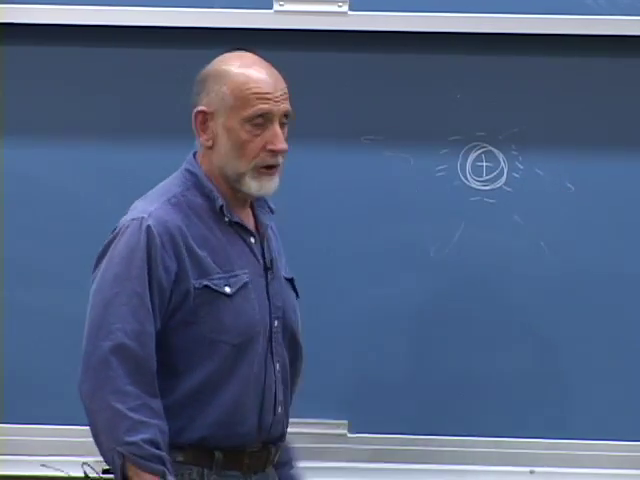
\includegraphics[width=0.82\textwidth]{lecture_10_figure_07.png}
\caption{在导体讨论中，一个源电荷被一团带相反电荷的屏蔽云所包围。}
\lectureframe{00:50:24}
\label{fig:l10-conductor-screening}
\end{figure}

\begin{classroomqa}
\audiencequestion{这种重新排布就是屏蔽的含义吗？\lecturetimestamp{00:51:25}}
\lecturerresponse{是的。在大于电荷云的尺度上，插入的电荷被屏蔽了。将另一个探针放入电荷云内部，一部分屏蔽电荷便不能再位于源与探针之间；此时底层的电荷显得更强。}
\end{classroomqa}

电荷云具有一个由可移动电荷的动力学和密度所设定的特征尺度。在小于该尺度的间距\(r\)处，探针会穿透电荷云。因此，可以通过下式定义一个跑动电荷\(e(r)\)
\begin{equation}
  F(r)\equiv\frac{e^2(r)}{4\pi r^2}.
  \label{eq:l10-running-charge-definition}
\end{equation}
对于理想化的导体，\(e(r)\)在极长距离处趋近于零，而在极短距离处趋近于微观值。

\subsection{电介质：部分屏蔽}

在绝缘体中，电子被束缚在原子周围，而不能自由地穿过样品。一个粗略但有用的模型将每个电子云描绘为通过一根弹簧与其离子相连。没有外场时，正负电荷中心的平均值重合。施加外场会使它们略微分开，并诱导出一个偶极子。

在负源周围，附近的电子云向外偏移，使其正离子略微更靠近；在正源周围，它们则向相反方向偏移。束缚电荷无法流动到足够远以完全中和源，因此长距离处的场被介电常数削弱，而不是被消除：
\begin{equation}
  V_{\mathrm{medium}}(r)
  =
  \frac{1}{\epsilon_r}
  \frac{e_1e_2}{4\pi\epsilon_0r}.
  \label{eq:l10-dielectric-coulomb}
\end{equation}
在极化云内部的间距处，探针再次看到更多裸源的贡献。完全屏蔽与部分屏蔽是同一个依赖于尺度的思想的两种版本。

\section{作为可极化介质的QED真空}

量子电动力学在其真空中没有物质原子，但它有带电的量子场。电子-正电子涨落为光子传播贡献圈图。在较旧的狄拉克海语言中，电场使填满的负能态发生畸变；在现代语言中，真空极化修饰了光子传播子。介质图像说的是，一个虚对被极化了：它的正、负分量向相反方向偏移。

正源周围有少量过剩的负极化电荷，而负源周围则有正极化电荷。因此，在远处测量到的电荷小于人们会与一个未被分辨的源联系起来的参数。与普通材料不同，真空包含遍及连续动量范围的涨落。低能对应对应于更长距离的结构；高能对则探测更短的距离。并不存在一个过程会就此停止的最终电荷云半径。

当两个电子被拉近时，最大的极化云首先不再能容纳于它们之间。将它们进一步拉近会依次剥离越来越小的云。有效电耦合随距离的倒数，或等价地随能量，呈对数增长：
\begin{equation}
  \alpha(Q)
  \simeq
  \frac{\alpha(\mu)}
  {1-\dfrac{2\alpha(\mu)}{3\pi}
  \ln\!\left(\dfrac{Q}{\mu}\right)}
  \label{eq:l10-qed-running}
\end{equation}
对于单个带电狄拉克费米子，在其阈值以上远高于阈值处，领头阶下如此。当越过其他带电粒子的阈值时，额外的带电种类会改变系数。

\begin{figure}[htbp]
\centering
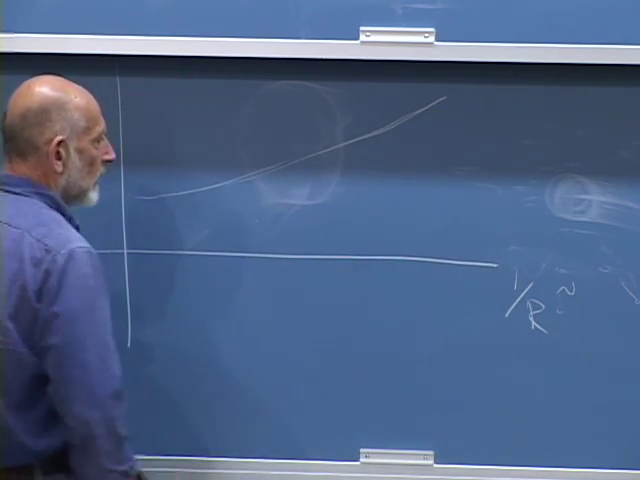
\includegraphics[width=0.82\textwidth]{lecture_10_figure_08.png}
\caption{QED有效电荷随着水平尺度\(1/R\)，因而也就是探测能量，的增加而缓慢上升。}
\lectureframe{01:02:13}
\label{fig:l10-qed-running-board}
\end{figure}

电子散射给出了可操作的版本。更高的碰撞能量意味着更短的德布罗意波长和更小的最近接近距离。因此，振幅必须使用与该动量转移相适配的耦合，而不是对所有能标都使用一个固定数值。

\begin{classroomqa}
\audiencequestion{在什么距离上，跑动才首次变得可测量？\lecturetimestamp{01:03:54}}
\lecturerresponse{电子真空极化在电子康普顿标度附近变得相关，\(\lambda_C=\hbar/(m_ec)\)，约化波长约为\(4\times10^{-11}\,\mathrm{cm}\)。该效应很小且是对数式的，因此需要精度。更重的带电粒子在各自的阈值处加入跑动。}
\end{classroomqa}

\begin{classroomqa}
\audiencequestion{谈论最小距离是否假设我们已经知道那里会发生什么？\lecturetimestamp{01:04:49}}
\lecturerresponse{不。我们只在该理论的粒子内容和相互作用仍然有效时才对其进行外推。新物理可以改变跑动。实验并没有告诉我们，QED在任意短的距离上仍然是完整的描述。}
\end{classroomqa}

\begin{classroomqa}
\audiencequestion{对于胶子，标度依赖是相反的吗？为什么？\lecturetimestamp{01:05:03}}
\lecturerresponse{是的。夸克圈以类似于带电物质的方式屏蔽色荷，但胶子本身带色并发生非线性相互作用。它们的贡献具有相反的符号，并且在观测到的夸克味数下占主导。其结果是反屏蔽和渐近自由。}
\end{classroomqa}

\begin{classroomqa}
\audiencequestion{如果确定裸电荷需要无限小的距离，那么人们如何能够确定它？\lecturetimestamp{01:05:28}}
\lecturerresponse{人们并不直接测量一个唯一的、与正规化无关的裸电荷。人们在选定的短距离截断或重整化标度处定义一个参数，然后调整它，使某个已测量的低能物理量保持不变。依赖于标度的重整化耦合才是有用的物理对象。}
\end{classroomqa}

\begin{classroomqa}
\audiencequestion{QED电荷在无限能量下会趋近一个有限值吗？\lecturetimestamp{01:05:39}}
\lecturerresponse{在单独外推的微扰QED中不会。其正的贝塔函数使耦合继续对数式增长，并在形式上导致一个出现在极高标度处的朗道极点。远在把那个形式上的极点当作物理之前，人们就预期该描述会被嵌入电弱理论，并最终被进一步的物理所改变。}
\end{classroomqa}

\subsection{重整化改变了什么，又保留了什么}

选择一个截断长度\(a\)，将相应的输入称为\(e(a)\)，并计算一个固定的长距离可观测量。另一个截断\(a'\)同样可以接受，只要将输入改为\(e(a')\)，使得同一个可观测量被重现：
\begin{equation}
  \frac{d}{d\ln\mu}\,\mathcal O_{\mathrm{physical}}=0,
  \qquad
  \mu\frac{de}{d\mu}=\beta(e).
  \label{eq:l10-rg-invariance}
\end{equation}
这种补偿性的流动就是重整化群。

\begin{classroomqa}
\audiencequestion{“裸”这个词必须特指普朗克长度吗？\lecturetimestamp{01:06:20}}
\lecturerresponse{不。人们可以在任何选定的截断处终止描述，并把那里的参数称为裸的。改变截断并相应地改变该参数，可使可及的物理保持不变。普朗克长度是普通量子场论必须被取代的一个可能位置，而不是重整化所要求的约定。}
\end{classroomqa}

\begin{classroomqa}
\audiencequestion{这个过程是否就是放大并削弱描述？\lecturetimestamp{01:07:15}}
\lecturerresponse{它在概念上是放大。我们问的是，一个更精细描述的参数必须如何改变，才能使在固定的、实验上可及的波长处的预言保持不变。}
\end{classroomqa}

\begin{classroomqa}
\audiencequestion{引力也会发生同样的跑动现象吗？\lecturetimestamp{01:08:14}}
\lecturerresponse{引力也有标度依赖，但并不简单地是同样的介电屏蔽机制。对于本讲来说，一个量纲论证就足够了：局域化提高能量，能量产生引力，而由此得到的无量纲引力强度随能量迅速增长。}
\end{classroomqa}

\section{QCD：反屏蔽、通量管与渐近自由}

在强子距离上，色电场线并不像电磁库仑场那样球对称地散开。胶子自相互作用把它们挤压成夸克与反夸克之间的一条狭窄管。如果该管具有近似固定的单位长度能量\(\sigma\)，那么
\begin{equation}
  V_{q\bar q}(r)
  \simeq
  -\frac{C_F\alpha_s(r)}{r}
  +\sigma r .
  \label{eq:l10-cornell-potential}
\end{equation}
在大的\(r\)下，线性项占主导。拉伸这对粒子会产生更多的管，就像拉一根太妃糖一样，能量随之增长，而不是趋于零。这就是故事中禁闭的一面。

\begin{figure}[htbp]
\centering
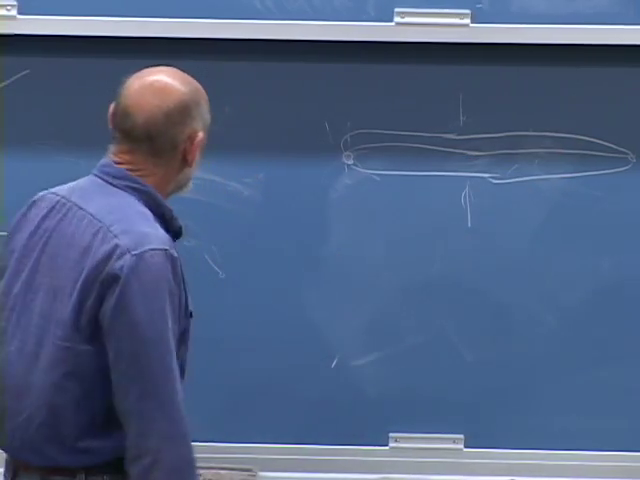
\includegraphics[width=0.84\textwidth]{lecture_10_figure_09.png}
\caption{色电场线被画成连接分离色源的管，而不是自由散开的库仑场。}
\lectureframe{01:09:56}
\label{fig:l10-qcd-flux-tube-board}
\end{figure}

在短于管半径的距离上，势近似回到库仑形式，但其耦合随能量减小。在一圈阶，
\begin{equation}
  \alpha_s(Q)
  =
  \frac{4\pi}
  {\left(11-\frac23n_f\right)
  \ln(Q^2/\Lambda_{\mathrm{QCD}}^2)} .
  \label{eq:l10-asymptotic-freedom}
\end{equation}
对于\(n_f<17\)，系数为正，且当\(Q\to\infty\)时\(\alpha_s(Q)\to0\)。QCD在极短距离上弱，在长距离上强。这正是讲座中相反行为的精确跑动耦合版本。

\begin{classroomqa}
\audiencequestion{在QED与QCD曲线之间的弱耦合会发生什么？\lecturetimestamp{01:11:53}}
\lecturerresponse{它的跑动是中间的，并且取决于跟踪的是哪个电弱因子。在电弱标度以上，恰当的物理量是\(U(1)_Y\)和\(SU(2)_L\)耦合。一个上升，另一个缓慢下降。与下降的强耦合一起，它们的外推值在很高能量下令人惊讶地接近。}
\end{classroomqa}

\section{跑向统一}

在弱标度附近测量三个规范耦合，并用所提出理论的粒子内容演化它们。因为每个贝塔函数都是对数式的，能量发生巨大变化只会引起耦合的适度变化。标准模型的轨迹彼此接近，但并不精确相交。对于最小超对称标准模型的低能粒子内容，一圈轨迹在
\begin{equation}
  M_{\mathrm{GUT}}\sim10^{16}\,\mathrm{GeV}.
  \label{eq:l10-gut-scale}
\end{equation}
附近更加接近地相交。

该图是证据，不是证明。来自未发现粒子的阈值、更高圈修正以及统一理论细节都会移动曲线。2010讲座强调超对称谱中大约百分级收敛，因为这使弱标度超对称特别有吸引力。如今对撞机能量下没有超伴侣，意味着该谱的最简单版本并未如最初预期那样实现；精确统一仍然依赖模型。

\begin{figure}[htbp]
\centering
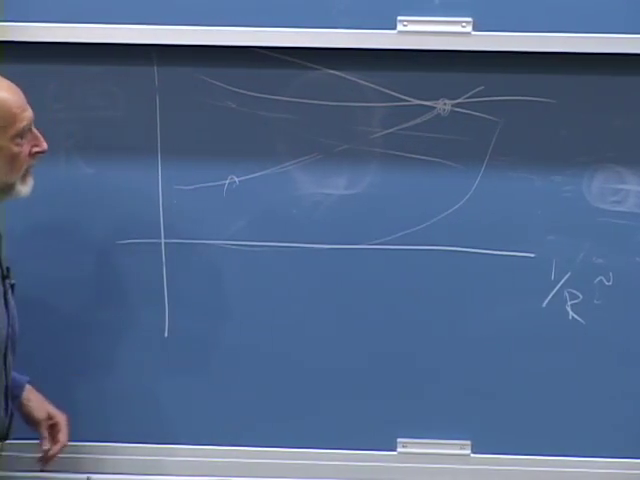
\includegraphics[width=0.84\textwidth]{lecture_10_figure_10.png}
\caption{黑板上的定性耦合图：强耦合曲线下降，电弱曲线缓慢向它演化，而引力在远紫外附近陡峭上升。}
\lectureframe{01:16:29}
\label{fig:l10-unification-board}
\end{figure}

为什么要把交点附近视为基本？因为在那里输入可能变得最简单。三个互不相关的低能耦合可能是同一个高能耦合的不同着装后代，而后者与单一规范群相关。这就是早先\(SU(5)\)问题背后的数值线索。

引力在同一张对数草图上表现为一条上升快得多的曲线。它并不恰好在GUT标度处穿过规范曲线，但在能量相差几个数量级之内就变成量级为一。在对数轴上，这种接近具有暗示性：\(10^{16}\)、\(10^{17}\)、\(10^{18}\)和\(10^{19}\,\mathrm{GeV}\)彼此之间远比它们中任何一个到电弱标度都更接近。

\section{为什么引力在短距离上增强}

\subsection{是能量，而不只是静质量，产生引力}

两个缓慢运动质量之间的牛顿力为
\begin{equation}
  F_G=\frac{Gm_1m_2}{r^2}.
  \label{eq:l10-newton-force}
\end{equation}
对于相对论性的量纲估计，把每个静质量替换为相应能量除以\(c^2\)：
\begin{equation}
  F_G(r)\sim\frac{GE_1E_2}{c^4r^2}.
  \label{eq:l10-relativistic-gravity-force}
\end{equation}
这不是广义相对论的替代；应力、动量流和压强也会作为引力源。它是针对当前问题的正确标度估计。

把每个粒子定域在大小为\(r\)的区域中。不确定性原理要求
\begin{equation}
  p\sim\frac{\hbar}{r}.
  \label{eq:l10-localization-momentum}
\end{equation}
在足够小的\(r\)下，动量是超相对论性的，所以
\begin{equation}
  E\simeq pc\sim\frac{\hbar c}{r}.
  \label{eq:l10-localization-energy}
\end{equation}
把两个这样的能量代入
\eqref{eq:l10-relativistic-gravity-force}
得到
\begin{equation}
  F_G(r)
  \sim
  \frac{G\hbar^2}{c^2r^4}.
  \label{eq:l10-short-distance-gravity-force}
\end{equation}
相应的势能标度为
\begin{equation}
  U_G(r)\sim-\frac{G\hbar^2}{c^2r^3}.
  \label{eq:l10-short-distance-gravity-potential}
\end{equation}
这就是现场计算中被纠正的区别：势按\(1/r^3\)标度，而力按\(1/r^4\)标度。

\begin{classroomqa}
\audiencequestion{对于超相对论性粒子，能量是
\(p^2/(2m)\)吗？\lecturetimestamp{01:22:18}}
\lecturerresponse{不是。那是非相对论公式。由
\(E^2=p^2c^2+m^2c^4\)，极限\(pc\gg mc^2\)给出
\(E\simeq pc\)。结合\(p\sim\hbar/r\)，定域化能量为
\(\hbar c/r\)。}
\end{classroomqa}

\begin{figure}[htbp]
\centering
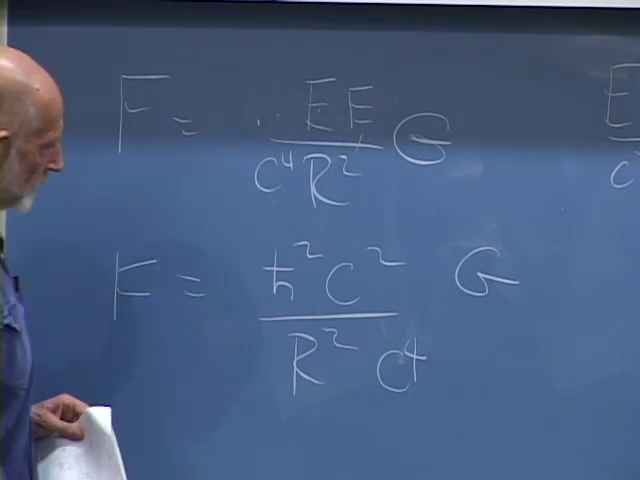
\includegraphics[width=0.84\textwidth]{lecture_10_figure_11.png}
\caption{黑板在检查\(c\)和\(r\)的幂次时，把相对论性能量代入牛顿定律。}
\lectureframe{01:23:29}
\label{fig:l10-gravity-derivation-board}
\end{figure}

\begin{classroomqa}
\audiencequestion{\(c\)的因子抵消了吗，并且所声称的
\(1/r^3\)定律是力定律吗？\lecturetimestamp{01:23:38}}
\lecturerresponse{黑板计算被实时纠正。两个有效质量贡献\(E_1E_2/c^4\)；在
\(E_i\sim\hbar c/r\)下，分母中留下两个\(c\)的幂次。得到的力是\(G\hbar^2/(c^2r^4)\)。\(1/r^3\)表达式属于势能。}
\end{classroomqa}

\begin{classroomqa}
\audiencequestion{这里讨论的引力是吸引的，对吗？\lecturetimestamp{01:24:42}}
\lecturerresponse{是的。上面的方程给出的是大小。对于正能量，牛顿引力势带有一个负号，因此在这个估计中力是吸引的。}
\end{classroomqa}

\begin{classroomqa}
\audiencequestion{引力是否因为局域化提高了能量而获得相对强度，而电荷本身却没有获得同样的运动学因子？\lecturetimestamp{01:25:02}}
\lecturerresponse{正是如此。能量就是引力荷。压缩一个量子态会提高其动量和能量，因此也会提高作为引力源的东西。电荷是无量纲的，不会获得那个直接的\(1/r\)因子，除了它慢得多的对数重整化之外。}
\end{classroomqa}

\subsection{普朗克交叉}

在自然单位下，量级为1的电荷之间的电磁力大小为
\begin{equation}
  F_{\mathrm{EM}}(r)
  \sim
  \alpha\,\frac{\hbar c}{r^2}.
  \label{eq:l10-em-force-alpha}
\end{equation}
将其与\eqref{eq:l10-short-distance-gravity-force}等同起来，得到
\begin{equation}
  r^2\sim\frac{G\hbar}{\alpha c^3}.
  \label{eq:l10-gravity-em-crossing}
\end{equation}
讲座将无量纲规范因子取为量级1，以揭示基本的引力长度：
\begin{equation}
  \boxed{\ell_P=\sqrt{\frac{\hbar G}{c^3}}}
  \simeq1.616\times10^{-35}\,\mathrm{m}.
  \label{eq:l10-planck-length}
\end{equation}
保留实际的\(\alpha\)会使与电磁学的等同关系移动一个量级1的对数尺度因子，\(r\sim\ell_P/\sqrt\alpha\)。基本陈述在自然单位下更为简洁：
\begin{equation}
\begin{aligned}
  \alpha_G(E)
  &\equiv\frac{GE^2}{\hbar c^5}
  =\left(\frac{E}{E_P}\right)^2,
  \\
  E_P
  &=\sqrt{\frac{\hbar c^5}{G}}
  \simeq1.22\times10^{19}\,\mathrm{GeV}.
\end{aligned}
  \label{eq:l10-gravitational-coupling}
\end{equation}
当\(E\)接近\(E_P\)时，引力变得强。

\begin{classroomqa}
\audiencequestion{在比较中，是\(G\)还是电耦合被设为1？\lecturetimestamp{01:27:02}}
\lecturerresponse{在粗略估计中，电耦合被当作量级1的数来处理。牛顿常数必须保留：它是决定普朗克尺度的有量纲量。}
\end{classroomqa}

\begin{classroomqa}
\audiencequestion{\(r\)、\(\hbar\)和\(c\)的中间幂次在量纲上并不一致。修正后的计算是什么？\lecturetimestamp{01:27:47}}
\lecturerresponse{从一开始就使用能量。局域化给出
\(E\sim\hbar c/r\)，因此
\(U_G\sim GE^2/(c^4r)=G\hbar^2/(c^2r^3)\)。将其与
\(U_{\mathrm{EM}}\sim\alpha\hbar c/r\)比较。将
\(\alpha\)设为量级1，得到
\(r^2=G\hbar/c^3\)。课堂和黑板上得到
\(r=\sqrt{G\hbar/c^3}\)，即普朗克长度。}
\end{classroomqa}

\begin{figure}[htbp]
\centering
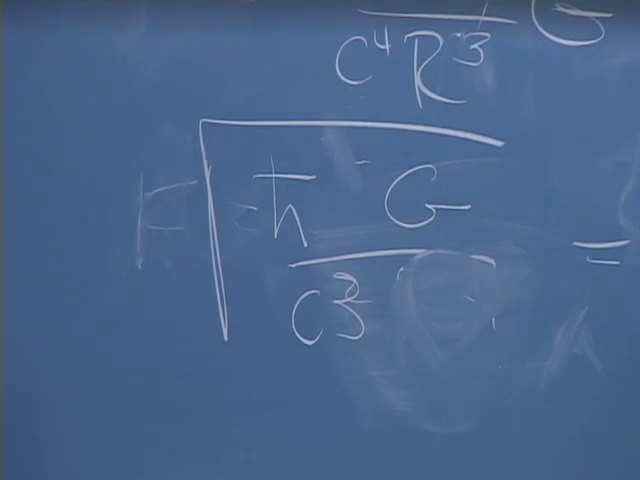
\includegraphics[width=0.84\textwidth]{lecture_10_figure_12.png}
\caption{现场量纲检验的修正终点：
\(r=\sqrt{\hbar G/c^3}\)。}
\lectureframe{01:32:16}
\label{fig:l10-planck-length-board}
\end{figure}

\section{等级问题重现}

规范耦合在一个非常高的尺度附近变得相当，而引力在普朗克尺度附近变得强。这些巨大的尺度现在看起来不那么像任意的大数，而更像微观描述可能简化的地方。与它们相比，电弱真空值\(F\)异常地小：
\begin{equation}
  \frac{v}{E_P}\sim2\times10^{-17}
  \label{eq:l10-electroweak-planck-ratio}
\end{equation}
在\(c=1\)的单位下。使用大统一尺度而非普朗克尺度会改变精确的比值，但不会改变这个谜题。

一旦\(F\)很小，\(W\)、\(Z\)、带电轻子和夸克的质量就随之而来，因为规范对称性使它们的质量与之成正比。没有这种保护的粒子可以保持很重。因此，突出的问题并不是为什么每个已知质量都独立地微小。而是为什么希格斯部门提供了这一个微小的对称破缺尺度。

\begin{classroomqa}
\audiencequestion{如果能够计算\(F\)，那么所有其他质量是否就可以计算了？\lecturetimestamp{01:34:39}}
\lecturerresponse{它将确定整体电弱尺度，并且在给定规范耦合和汤川耦合的情况下，确定相应的粒子质量。剩下的问题是，一个普通的对紫外敏感的计算倾向于将希格斯质量参数推向高基本尺度，除非有对称性或动力学机制保护它。}
\end{classroomqa}

“精细调节”一词预示了这种敏感性。在截断描述中，标量质量参数会收到大致形式的修正
\begin{equation}
  \delta\mu^2
  \sim
  \frac{C}{16\pi^2}\Lambda^2,
  \label{eq:l10-higgs-quadratic-sensitivity}
\end{equation}
其中\(C\)组合了规范、汤川和标量耦合，而\(\Lambda\)标记了有效理论被替换的尺度。如果
\(\Lambda\)接近大统一尺度或普朗克尺度，那么要得到
\(\mu^2\sim v^2\)似乎需要输入贡献与辐射贡献之间非常精确的抵消。这就是规范等级问题的自然性形式。它是对讲座承诺在下一季度进行的计算的编辑性补全，而不是声称某个特定的正规化方案人为产物本身是可观测的。

\begin{classroomqa}
\audiencequestion{普朗克长度是否应该被想象为最终的屏蔽云半径？\lecturetimestamp{01:35:03}}
\lecturerresponse{不。介电图像解释了规范荷的重整化，但普朗克论证使用的是局域化能量和有量纲的引力耦合。在这个推导中并没有字面意义上的引力屏蔽云。}
\end{classroomqa}

\subsection{关于相互作用的收尾问题}

最后几分钟回到希格斯势以及拉格朗日量可以包含哪些项。

\begin{classroomqa}
\audiencequestion{希格斯势能否包含\(\phi^6\)而仍然保持对称？\lecturetimestamp{01:35:20}}
\lecturerresponse{能。偶次幂保持玩具\(\phi\mapsto-\phi\)对称性，而\(\phi^5\)会破坏它。在四维中，\(\phi^6\)的系数具有负质量量纲，因此该项被高能标所压低，例如\(c_6\phi^6/\Lambda^2\)。它是一个有效的相互作用，尽管它不是幂次计数可重整的。}
\end{classroomqa}

\begin{classroomqa}
\audiencequestion{希格斯场的幂是否代表产生和湮灭过程，因此\(\phi^4\)预言希格斯-希格斯散射？\lecturetimestamp{01:35:52}}
\lecturerresponse{是的。在真空附近展开后，量子化场的幂产生顶点。四次项包含一个四希格斯顶点，而平移后的势也产生三次相互作用。知道它们的系数就能预言诸如\(hh\to hh\)的过程，前提是进行通常的费曼图计算。}
\end{classroomqa}

\begin{classroomqa}
\audiencequestion{基本拉格朗日量必须在其场中是多项式的，且没有高于四次的幂吗？\lecturetimestamp{01:36:09}}
\lecturerresponse{对于微扰可重整的四维标量理论，量纲至多为四的算符构成传统的有限列表。现代有效场论则不那么严格：允许更高量纲的算符，它们编码短距离物理，但其效应被高能标的幂所压低。因此，偶尔的例外对旧规则至关重要。}
\end{classroomqa}

\begin{classroomqa}
\audiencequestion{在关于跑动耦合的讨论中，自相互作用项被省略了吗？\lecturetimestamp{01:36:44}}
\lecturerresponse{它们在概念上已被包含。胶子自相互作用正是相对于QED反转符号并产生反屏蔽的原因。希格斯自相互作用同样对希格斯标量及其他标准模型参数的跑动有贡献。}
\end{classroomqa}

\begin{classroomqa}
\audiencequestion{是否存在不同相互作用彼此影响对方跑动的交叉项？\lecturetimestamp{01:37:23}}
\lecturerresponse{是的。在更高圈阶，贝塔函数包含规范耦合、汤川耦合和标量耦合的混合乘积。只要这些无量纲耦合足够小，微扰论就仍然有用，因为逐阶圈阶相应地受到压低。}
\end{classroomqa}

\begin{classroomqa}
\audiencequestion{说\(F\)被精细调节究竟是什么意思？\lecturetimestamp{01:37:44}}
\lecturerresponse{完整的答案在讲座中被推迟了。问题在于轻标量能标相对于大得多的紫外贡献的不稳定性，这由\eqref{eq:l10-higgs-quadratic-sensitivity}概括。超对称是所提出的一种强制抵消的方式，但等级问题本身并不选择出一个已确认的解决方案。}
\end{classroomqa}

\begin{classroomqa}
\audiencequestion{现在能解释重整化群本身吗？\lecturetimestamp{01:37:56}}
\lecturerresponse{在剩下的几分钟里不能。它的操作性内容已经出现过了：改变分辨率，让耦合跑动，并保持固定的物理预言。完整的处理属于课程的下一阶段。}
\end{classroomqa}

这就是这一序列恰当地留给我们的地方。希格斯机制使标准模型在内部自洽：它保持手征规范对称性，赋予弱规范玻色子和费米子质量，并预言物理的希格斯相互作用。重整化随后教给我们这些相互作用如何随能标变化，并暗示规范力可能有一个统一的起源。引力通过一个独立的论证提供了第二个高能标。这些成功都没有解释为什么希格斯真空期望值远低于两者。因此，最后一讲并没有结束这个主题；它指出了下一个主题必须集中关注的那个小数字。